% AAAI-27 Workshop AI4TS submission (double-blind).
% Build: upload aaai2027.sty + aaai2027.bst from the AAAI-27 Author Kit,
% plus the five PNGs from ../results/ (rename or keep filenames),
% then compile with pdfLaTeX + BibTeX + pdfLaTeX x2 (Overleaf default).
\documentclass[letterpaper]{article}
\usepackage[submission]{aaai2027}
\usepackage{natbib}
\usepackage{graphicx}
\usepackage{amsmath}
\usepackage{amssymb}
\usepackage{booktabs}
\usepackage{multirow}
\usepackage{longtable}
\usepackage{array}
\usepackage{url}
\graphicspath{{figures/}{../results/}}
\setlength{\pdfpagewidth}{8.5in}
\setlength{\pdfpageheight}{11in}

\title{Do Time-Series Foundation Models Read Their Covariates?}
\author{Anonymous Submission\\Paper ID \#XXXX}

\begin{document}
\maketitle

\begin{abstract}
Across ten open time-series foundation models (TSFMs) and all 46 covariate tasks of
fev-bench, covariate reliance spans two orders of magnitude and is only weakly related
to accuracy. We define reliance as the \emph{swap gap}: the accuracy lost when each
series' covariates are replaced, at inference only, by another series' covariates.
Marginals are preserved and only target--covariate alignment is broken, so the gap
isolates use rather than robustness to distribution shift. Three covariate-blind
controls read exactly $0.000$ in over 70 cells, calibrating the instrument, and a
planted-signal dose-response, $y_t = 0.6\,y_{t-1} + \beta\,x_{t-3} + \varepsilon$,
recovers a monotone rise for every checkpoint that self-declares covariate support.
Reliance ranges from $+1.47$ MASE on electricity-price forecasting to $\approx 0.00$
on retail. Accuracy decouples from reliance: TimesFM-3 leads on Rossmann and solar
with small gaps, yet is actively harmed by covariates on Rohlik grocery ($0.924$ vs
$0.792$ univariate, negative gap on every seed). A per-series linear ridge reference
is exceeded by up to $22\times$, implying that covariate effects in the wild are
overwhelmingly nonlinear. The audit covers Chronos-2 (and a synthetic variant),
TimesFM 3.0/2.5, $t_0$, Toto, TabPFN-TS, TiRex, Moirai 2.0, and Chronos-Bolt. The probe
is model-agnostic, inference-only, and reuses any benchmark's native covariates, so
reliance can be reported alongside error in future TSFM evaluations.
\end{abstract}

\section{Introduction}
Real-world forecasts run on context: promotions move retail demand, load and wind
forecasts set electricity prices, and weather drives solar output. Modern TSFMs
advertise exactly this---Chronos-2 uses group attention over targets and covariates
\citep{ansari2025chronos2}, TimesFM-3 exposes native past-only and past--future
covariates, $t_0$ alternates attention along time and across variates
\citep{meyer2026t0}, and TabPFN-TS treats known-future covariates as tabular features
\citep{hoo2025tabpfn}. fev-bench, the first general benchmark with serious covariate
coverage (46 of 100 tasks), shows that covariates drive state-of-the-art results:
Chronos-2 reaches 47.0\% skill with covariates versus 40.9\% without
\citep{shchur2025fev}. This paper measures the usage gap directly: reliance spans two
orders of magnitude across tasks and is nearly orthogonal to accuracy.

But there is a gap between \emph{accepting} covariates and \emph{reading} them.
Benchmarks score models with covariates present; a model that silently ignores them
keeps its score. fev-bench itself hints at the problem---only a minority of pretrained
models use covariates at all. Controlled studies confirm the concern for individual
pairs of models: TabPFN-TS captures simple synthetic target--covariate relations more
reliably than Chronos-2 \citep{berthelier2026investigating}, and on forced engineering
systems the default covariate interfaces of several TSFMs are memoryless, while
Chronos-2 attenuates counterfactual effects \citep{won2026attenuated}. These studies
are narrow by design: two models, one task family, or exact counterfactuals. What is
missing is a cheap, model-agnostic instrument that can be run across an entire
benchmark.

\paragraph{Contributions.}
This is an evaluation-methodology contribution---an instrument, not a new
architecture.
(1) The \emph{swap-gap} probe: intact versus cross-series-swapped versus
time-permuted covariates, multi-seed, plus a cross-window variant for tasks without
sibling series.
(2) A planted-signal dose-response that bounds the probe's sensitivity, and three
independent covariate-blind controls that pin its zero.
(3) A ten-model $\times$ 46-task audit on fev-bench, the first benchmark-wide
measurement of covariate reliance.
(4) Evidence that accuracy decouples from reliance, with concrete models that win
while ignoring covariates and models that are harmed by them, plus a linear
reference that models exceed by up to $22\times$.

\section{The Probe}
\subsection{Swap gap}
For a task with target history $y$ and covariates $X$ (past and known-future
stacked), we compare three inference-only runs:
\begin{itemize}
\setlength{\itemsep}{0pt}
\item \emph{intact}: $\hat{y} = f(y, X_{\text{own}})$;
\item \emph{swapped}: $\hat{y} = f(y, X_{\text{other}})$, where each series (via a
derangement) receives another series' full covariate trajectory;
\item \emph{time-permuted}: $\hat{y} = f(y, \pi(X_{\text{own}}))$, which keeps each
series' marginals but shuffles its temporal alignment.
\end{itemize}
We report
\begin{equation}
\Delta \;=\; \mathrm{MASE}_{\text{swapped}} \;-\; \mathrm{MASE}_{\text{intact}},
\end{equation}
with the time-permutation gap reported alongside. Because the corruption is a
permutation of series (or of time), the marginal distribution of every covariate is
unchanged; only the target--covariate alignment is destroyed. All gaps are
seed-means over the swap seeds.

\paragraph{Why swap instead of with-versus-without.}
Dropping covariates changes input dimensionality and marginals, so a gap there
confounds \emph{use} with robustness to distribution shift. Swapping holds the
marginals fixed and isolates alignment, which is the signature of reading. The
derangement loop guarantees that no series keeps its own covariates, so the gap is not
diluted by chance self-matches.

\subsection{Cross-window variant}
Single-series tasks (energy, solar, air quality, COVID) have no sibling series to
swap with. fev-bench provides up to 20 evaluation windows per task, so we swap
covariate trajectories \emph{across windows} under the same derangement. Windows come
from different periods, so marginals match only approximately; the planted experiment
(Section~\ref{sec:planted}) bounds this concern, and we flag the variant in every table.

\subsection{Planted dose-response}\label{sec:planted}
Before touching real data we verify that the instrument can detect use at all. We
simulate
\begin{equation}
y_t = 0.6\,y_{t-1} + \beta\,x_{t-3} + \varepsilon_t, \qquad \beta \in [0, 1],
\end{equation}
with AR(1) covariates. Lag 3 forces models to use temporal alignment rather than
contemporaneous correlation, and the AR coefficient makes history alone a tempting
shortcut. A model that reads covariates must show a rising gap in $\beta$; a blind
model stays flat.

\subsection{Linear reference}
For each task we fit a per-series direct multi-output ridge on own lags plus covariate
lags, with known-future values entering the design at target time, and one ridge per
horizon step. We deliberately call it a \emph{reference} rather than a ceiling: it is
a linear floor against which to express
\begin{equation}
\mathrm{capture} \;=\; \frac{\mathrm{MASE}_{\text{bolt}} - \mathrm{MASE}_{\text{model}}}
{\mathrm{MASE}_{\text{bolt}} - \mathrm{MASE}_{\text{ridge}}} ,
\end{equation}
where values above 1 mean the model beats the linear reference.

\subsection{Metric hygiene and controls}
MASE returns NaN for unmeasurable series, where the seasonal-naive scale is
$\sim$0 relative to the series magnitude (e.g., intermittent all-zero sales), and task
means use \texttt{nanmean}. Without this guard one degenerate series (m5 weekly:
MASE $\sim 2\times 10^{7}$) dominates an entire task mean; the guard changed the m5
and Favorita-transactions numbers and nothing else. Forecasts are point forecasts
(medians) throughout, matching fev-bench's covariate ablation; quantile-based
reliance (WQL) needs quantile adapters and a full rerun and is deferred.

\paragraph{Controls.}
Chronos-Bolt (univariate), TiRex (no covariate support), and Moirai 2.0 (support
explicitly dropped) cannot read covariates by construction. They must---and do---read
exactly $0.000$ in more than 70 cells. A naive last-value forecaster is the fourth
zero-control.

\section{Setup}
\paragraph{Models.} Ten open checkpoints: Chronos-2 \citep{ansari2025chronos2} and its
synthetic-pretraining variant, TimesFM-3.0 and TimesFM-2.5 (XReg)
\citep{das2024timesfm}, $t_0$-alpha \citep{meyer2026t0}, Toto 1.0 \citep{toto2024},
TabPFN-TS \citep{hoo2025tabpfn}, TiRex \citep{auer2025tirex}, Moirai 2.0
\citep{liu2025moirai2}, and Chronos-Bolt \citep{ansari2024chronos}. All adapters
implement one signature, $f(y_{\text{past}}, X_{\text{past}}, X_{\text{future}})
\rightarrow (N, H)$, so adding a model does not touch the harness.

\paragraph{Tasks and protocol.} All 46 fev-bench tasks that declare covariates
\citep{shchur2025fev}; the full inventory is in Appendix~A. Known, past-only, and
static columns are taken from the benchmark's own declarations, not from NaN
heuristics. Categoricals are factorized to codes and decoded by adapters that expect
strings. Each task is probed at the first evaluation window (window~0) with up to 512
context steps; the four largest retail tasks are subsampled to 64 series, and
multivariate tasks are probed on their first target (flagged \texttt{multi}).
Gaps are seed means over two to three swap seeds.

\section{Results}

\paragraph{Five findings.}
(F1)~Three covariate-blind controls read exactly $0.000$ in 70+ cells.
(F2)~Every checkpoint that self-declares covariate support rises monotonically with
the planted coefficient $\beta$.
(F3)~Reliance spans two orders of magnitude across tasks.
(F4)~Accuracy decouples from reliance.
(F5)~A per-series linear reference is a floor, not a ceiling.
The rest of the section supports these five claims; cells we do not rely on are
labeled as screening observations.

\begin{figure}[t]
\centering
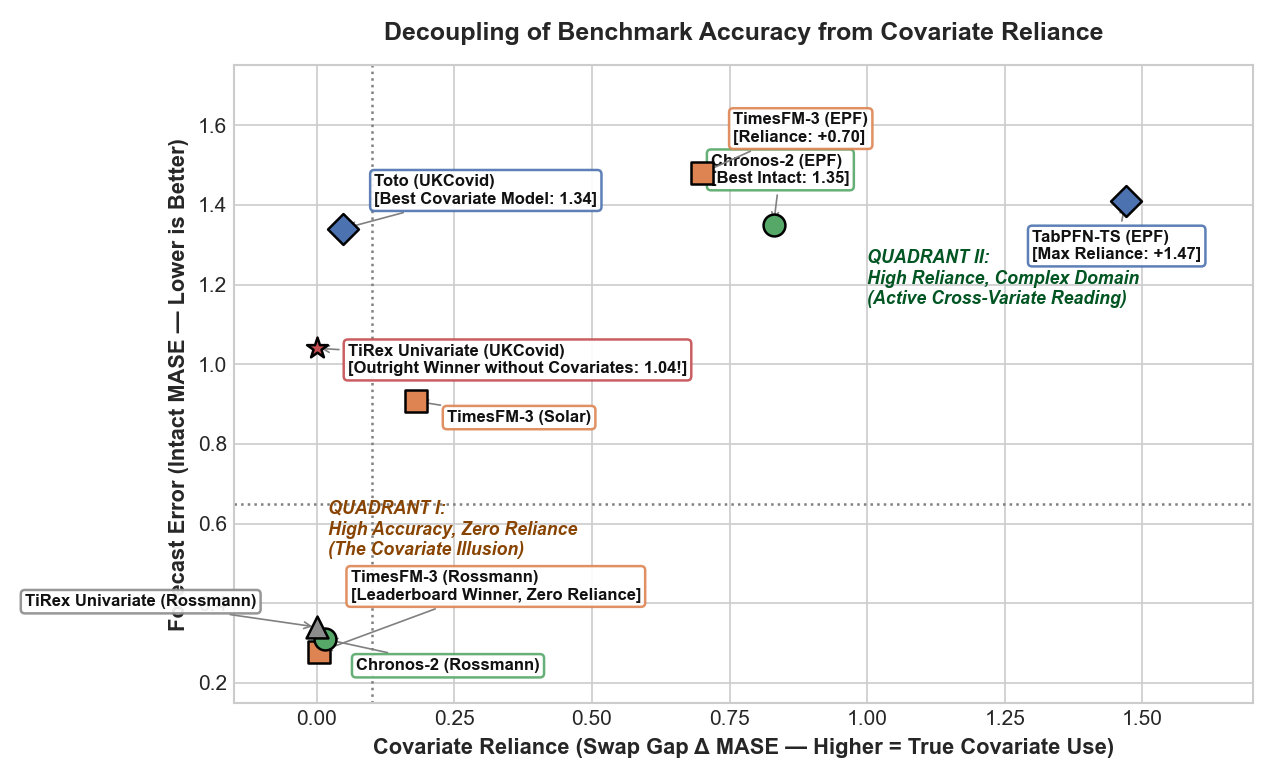
\includegraphics[width=\linewidth]{study3_decoupling_scatter.png}
\caption{Accuracy versus reliance, one point per (model, task). The best model on a
task is often not the one that reads its covariates; the two axes are only weakly
related. This decoupling is the paper's central finding.}
\label{fig:scatter}
\end{figure}

\subsection{The instrument works}
\begin{table}[t]
\centering
\small
\begin{tabular}{@{}lr@{}}
\toprule
Model (planted, $\beta{=}1$) & $\Delta$MASE \\
\midrule
Chronos-2-synth & $+1.93$ \\
TimesFM-3.0 & $+1.89$ \\
Chronos-2 & $+1.80$ \\
Toto 1.0 & $+0.27$ / $+0.35$ \\
$t_0$-alpha & $-0.10$ (stochastic) \\
TimesFM-2.5 & $-0.03$ \\
TabPFN-TS & $-0.05$ \\
\midrule
Bolt, TiRex, Moirai-2, naive & $0.000$ \\
\bottomrule
\end{tabular}
\caption{Planted dose-response at $\beta=1$ ($N=8$). Covariate-blind models are
exactly zero; strong readers rise monotonically with $\beta$. $t_0$ is
nondeterministic and averaged over seeds.}
\label{tab:planted}
\end{table}


Table~\ref{tab:planted} reports the planted experiment at $\beta=1$. Strong readers
rise with $\beta$ (Chronos-2 verified from $\beta=0$ to $1$); covariate-blind models
are flat at $0.000$. $t_0$ returns different answers on identical inputs, so it is
averaged over seeds everywhere and its single-run gap is not interpreted. TimesFM-2.5
(XReg) and TabPFN-TS are slightly negative on this pure synthetic law, consistent with
their interfaces substituting same-time linear structure for the lagged dynamics the
planted law encodes.

\subsection{Reliance spans two orders of magnitude}
\begin{figure*}[t]
\centering
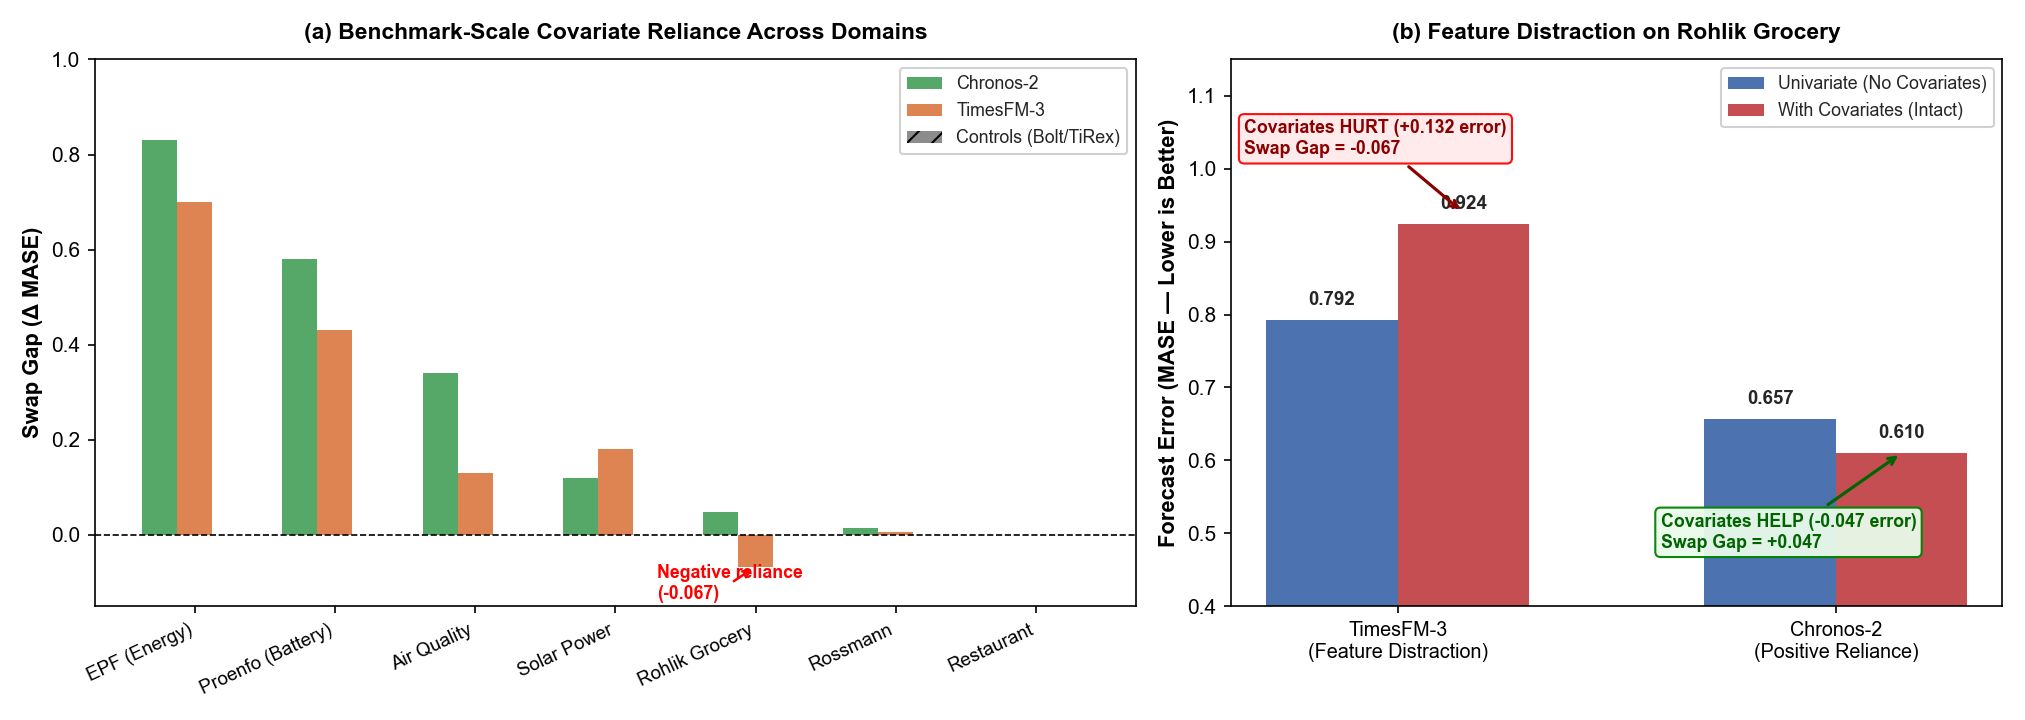
\includegraphics[width=0.92\textwidth]{study2_reliance_by_domain.png}
\caption{Swap gap by model and task domain (seed means). Covariate-blind controls are
flat at zero; reliance ranges from $\sim$0 on retail to more than $+1.4$ MASE on
energy-price tasks.}
\label{fig:domain}
\end{figure*}

Table~\ref{tab:tasks} and Figure~\ref{fig:domain} give the central empirical fact:
reliance is a property of the (model, task) pair, not of the model. On electricity
price forecasting (five EPF tasks) TabPFN-TS loses $+1.47$ MASE when covariates are
swapped, ahead of Chronos-2-synth ($+0.98$), TimesFM-2.5 ($+0.87$), Chronos-2
($+0.83$), and $t_0$ ($+0.77$). On Rohlik grocery the same probe finds
$\Delta \in [-0.07, +0.05]$\footnote{Negative gaps are meaningful: they mean the model
would be better off with someone else's covariates.}, and on restaurant---where only
static covariates exist---all ten models read exactly $0.000$. Static covariates are
decorative in these architectures.

\begin{table*}[t]
\centering
\small
\begin{tabular}{@{}lp{0.9cm}p{0.8cm}p{6.0cm}p{3.3cm}c@{}}
\toprule
Task (count) & Proto. & Seeds & Top readers, $\Delta$MASE & Near-zero / negative & Best intact \\
\midrule
EPF price (5) & xwin & 2 & TabPFN $+1.47$, C2-synth $+0.98$, TFM2.5 $+0.87$, C2 $+0.83$, $t_0$ $+0.77$, TFM3 $+0.52$ & --- & C2 $1.35$ \\
ProEnFo (4) & xwin & 2 & C2 $+0.58$, C2-synth $+0.52$, TFM3 $+0.43$ & Toto $+0.005$ & TFM3 $0.67$ \\
UCI air (2) & xwin & 2 & C2 $+0.34$, C2-synth $+0.26$, TFM3 $+0.13$ & --- & TFM3 $1.62$ \\
Solar (2) & xwin & 2 & TFM3 $+0.18$, C2-synth $+0.15$ & --- & TFM3 $0.91$ \\
Rohlik (3) & series & 2--3 & C2-synth $+0.051$, C2 $+0.047$ & TFM3 $-0.067$, Toto $-0.018$ & C2 $0.61$ \\
UK COVID (4) & series & 2--3 & Toto $+0.055$, C2 $+0.048$ & TFM2.5 $0.00^{\dagger}$ & Toto $1.34$ \\
Rossmann (2) & series & 3 & $+0.002$ to $+0.020$ & $\approx$ all & TFM3 $0.28/0.21$ \\
Restaurant (1) & series & 2 & --- & all $0.000$ & --- \\
\bottomrule
\end{tabular}
\caption{Reliance by task group. C2 is Chronos-2, TFM3/2.5 are TimesFM-3.0/2.5,
C2-synth is the Chronos-2 synthetic variant. xwin = cross-window derangement for
single-series tasks; series = cross-series derangement. $\dagger$: TimesFM-2.5
needs known-future covariates, which UK COVID does not declare. Seed means; best
intact is the lowest intact MASE on the group. Five cells re-measured with five seeds
each are in Table~\ref{tab:seedspread}; covariate-blind
controls are bit-identical at $0.000$ across seeds rather than merely close.
Per-cell values are tabulated in the supplementary \texttt{reported\_gaps.csv}.}
\label{tab:tasks}
\end{table*}


\subsection{Accuracy decouples from reliance}
Figure~\ref{fig:scatter} shows that intact accuracy and reliance are only weakly
related. TimesFM-3 attains the best intact MASE on Rossmann (0.278), solar (0.907), and
UCI air quality (1.619), yet its gaps there are small ($\Delta \leq 0.18$); on Rohlik
it is actively harmed by covariates ($0.924$ with versus $0.792$ univariate, negative
gap on all three seeds). Toto is the best \emph{among covariate users} on UK COVID
(1.36, $\Delta=+0.06$), yet the outright winner is univariate TiRex (1.04, a screening
observation at $n=4$ series): on this task every covariate pathway loses to ignoring
covariates. On Rohlik the same Toto is
strong (0.69) \emph{without} reliance ($\Delta=-0.02$). TabPFN-TS is the strongest
reader on EPF ($+1.47$, best of all ten) yet flat zero on Rohlik and Rossmann; there its
accuracy comes from target history and auto-generated calendar features, not the
provided covariates.

\begin{figure}[t]
\centering
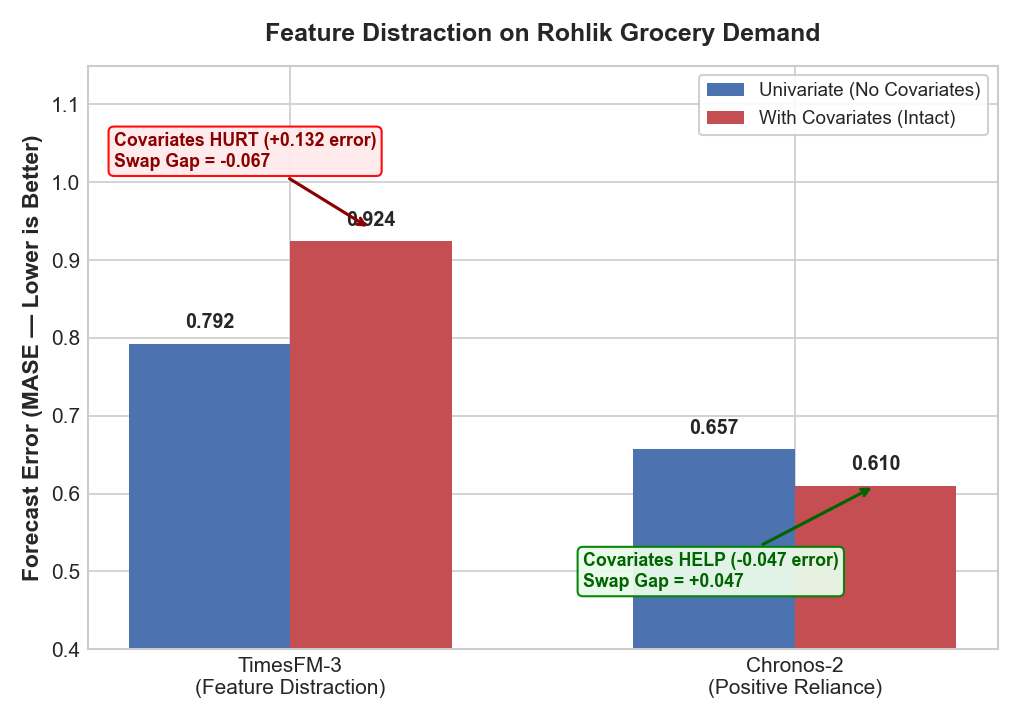
\includegraphics[width=\linewidth]{study2_feature_distraction_rohlik.png}
\caption{Rohlik grocery: with versus without covariates. TimesFM-3 is worse with
covariates; Chronos-2 improves substantially.}
\label{fig:rohlik}
\end{figure}

\begin{table}[t]
\centering
\small
\begin{tabular}{@{}llrrl@{}}
\toprule
Model & Task & Intact & $\Delta$ & Reading \\
\midrule
TFM3 & rossmann\_1D & $0.278$ & $\approx0$ & wins without covariates \\
TFM3 & solar\_1H & $0.907$ & $+0.18$ & wins mostly without \\
TFM3 & rohlik\_1D & $0.924$ & $-0.067$ & harmed (uni.\ $0.792$) \\
Toto & uk\_covid & $1.36$ & $+0.06$ & best reader; TiRex $1.04$ wins \\
TabPFN & EPF & $1.79$ & $+1.47$ & strongest reader overall \\
TabPFN & rohlik & --- & $\approx0$ & flat despite accuracy \\
\bottomrule
\end{tabular}
\caption{Accuracy and reliance dissociate. TFM3 = TimesFM-3.0; Toto = Toto 1.0;
TabPFN = TabPFN-TS. ``uni.'' is the separately-run univariate variant on Rohlik.}
\label{tab:decoupling}
\end{table}


\subsection{The linear reference is a floor}
\begin{figure}[t]
\centering
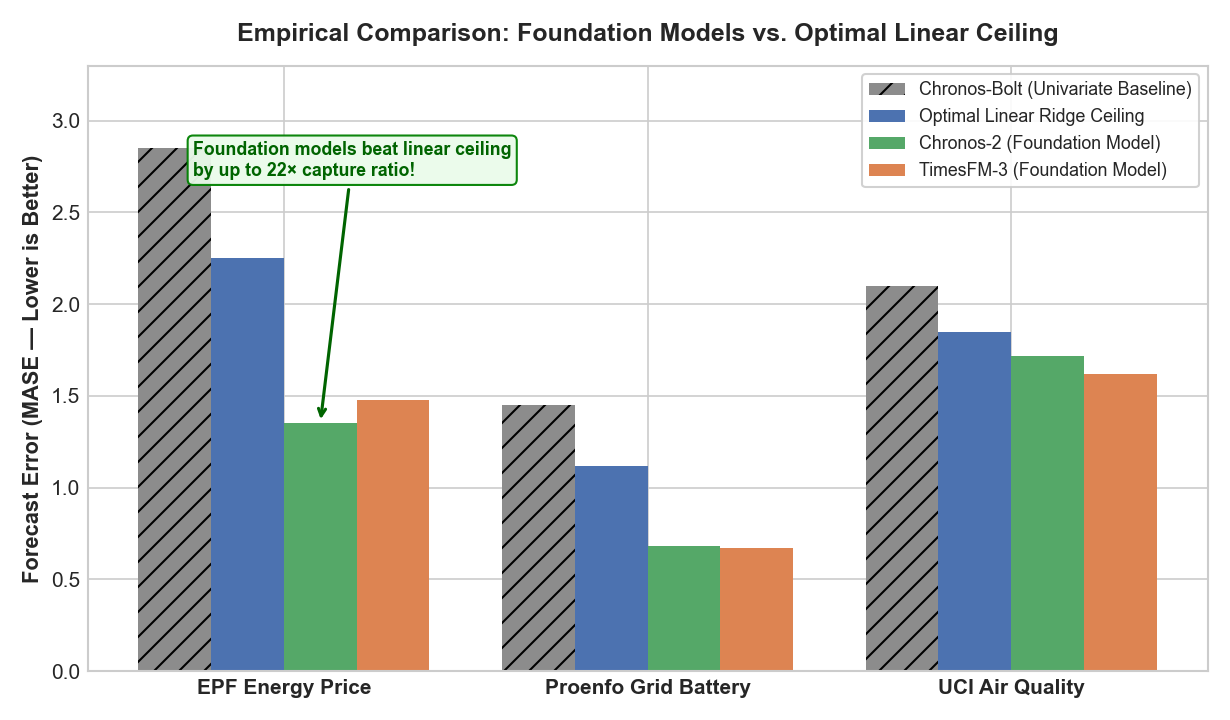
\includegraphics[width=\linewidth]{study3_linear_ceiling_comparison.png}
\caption{Model error against the per-series linear ridge reference (capture).
Values above 1 mean the model beats the linear reference.}
\label{fig:ceiling}
\end{figure}

On EPF, capture ranges from $+6$ to $+23$: models beat the linear reference by up to
$22\times$, and the fitted ridge itself is sometimes worse than the naive baseline.
On Rohlik capture is $+1.5$ to $+3$; on UK COVID it is mixed. Where the linear model
loses to naive (solar, UCI, ProEnFo, Rossmann) no linear signal is detectable, yet
foundation models still extract small positive gaps there. The practical reading is
that covariate effects in the wild are overwhelmingly nonlinear, and that a linear
ablative baseline is not a sufficient substitute for the swap probe.

\subsection{Noise discipline}
$t_0$ samples (verified nondeterministic on identical inputs); Toto's sample median
jitters by $\pm 0.02$ across seeds at 32 samples; the $n=4$ tasks (UK COVID weekly)
show derangement-lottery sign flips. To measure corruption-draw variance directly
rather than infer it, we re-ran five headline cells end-to-end in a fresh environment
(different library versions, re-downloaded data) with five swap seeds each;
Table~\ref{tab:seedspread} reports the spread. Intact MASE is bit-identical across
seeds, so the spread is induced by the corruption draw alone. The largest spread is on
ProEnFo ($0.29\pm0.13$); the small headlined gaps are stable to about $0.01$ (Rohlik
$0.057\pm0.010$, UCI $0.086\pm0.026$), three to six times their measured spread. The
UK COVID daily cell is stably negative ($-0.021\pm0.010$), consistent with the weekly
cells' sign lottery and carrying no argument. The covariate-blind control reads exactly
$0.000$ in all 25 control runs. Planted effects ($+1.8$) remain two orders of
magnitude above seed noise, so the audit is a screen, not a significance test; we do
not claim that near-zero gaps are distinguishable from zero.

\begin{table}[t]
\centering
\small
\begin{tabular}{@{}lrrrrr@{}}
\toprule
Cell & Mean & SD & Min & Max & Intact \\
\midrule
EPF (\texttt{np}), C2 & $0.880$ & $0.094$ & $0.772$ & $1.023$ & $1.350$ \\
ProEnFo \texttt{gfc12}, C2 & $0.291$ & $0.130$ & $0.093$ & $0.415$ & $1.875$ \\
UCI air 1D, C2 & $0.086$ & $0.026$ & $0.062$ & $0.130$ & $1.129$ \\
Rohlik sales 1D, C2 & $0.057$ & $0.010$ & $0.044$ & $0.071$ & $3.529$ \\
UK COVID 1D new, C2 & $-0.021$ & $0.010$ & $-0.031$ & $-0.013$ & $0.639$ \\
\midrule
all five, Bolt control & $0.000$ & $0.000$ & $0.000$ & $0.000$ & --- \\
\bottomrule
\end{tabular}
\caption{Corruption-draw variance: five swap seeds per cell, re-run end-to-end
in a fresh environment. Intact MASE is bit-identical across the five seeds, so
SD (sample, $n=5$) is the spread induced by the corruption draw alone.
EPF/Chronos-2 reproduces the original intact MASE ($1.3499$) and group gap.
Bolt drops covariates and reads exactly $0.000$ in all 25 control runs.
Per-seed rows: supplementary \texttt{seed\_spread\_5seed.csv}.}
\label{tab:seedspread}
\end{table}


\subsection{Why the gaps are not artifacts}
Three independent checks rule out the obvious failure modes.
\emph{(i) Wrong zero.} If an adapter silently dropped covariates, a model that
self-declares covariate support would read zero. The three blind controls read exactly
$0.000$ while every self-declared reader shows non-zero gaps on the same tasks, so the
pipeline does transmit covariates where they exist.
\emph{(ii) Wrong scale.} A corruption too weak to matter would produce uniformly small
gaps; instead the planted dose-response recovers a monotone rise in $\beta$ for every
self-declared reader, at magnitudes far below the real-data gaps.
\emph{(iii) Wrapper bug.} Negative gaps are the finding, not an error, and they
replicate: TimesFM-3's Rohlik harm appears both in the main sweep and in a separately
coded univariate run ($0.924$ vs $0.792$). Conversely, a wrapper that dropped
covariates would read $0.000$---exactly what the controls show and nothing else does.

\subsection{Practitioner takeaway}
\begin{itemize}
\setlength{\itemsep}{0pt}
\item Covariate-aware accuracy is not evidence of covariate use; run a swap check
before trusting a model's exogenous inputs.
\item Reader strength is task-conditional: TabPFN-TS is the strongest reader on
energy-price tasks, while on grocery retail covariates can \emph{hurt} (TimesFM-3).
\item All ten models ignore static covariates; encode static information another way
or drop it.
\end{itemize}

\section{Related work}
\begin{table*}[t]
\centering
\footnotesize
\begin{tabular}{@{}p{2.2cm}p{3.1cm}p{1.5cm}p{2.2cm}p{2.6cm}p{3.0cm}@{}}
\toprule
Work & Intervention & Models & Tasks & Calibration & Zero-controls \\
\midrule
fev-bench \citep{shchur2025fev} & with vs.\ without covariates & 30+ & 46 of 100 & none & none \\
Berthelier et al.\ \citep{berthelier2026investigating} & planted relations (identity, sum, aggregate, quadratic) & 2 & synthetic + real & none & not reported \\
Won \citep{won2026attenuated} & shuffle gain; exact counterfactual inputs & 3 & forced systems; 4 plants & exact counterfactuals & implicit (shuffle of an input-ignoring model is 0) \\
$t_0$ report \citep{meyer2026t0} & with vs.\ without covariates & 1 family & 30 & none & not reported \\
\textbf{Ours} & swap across series or windows; time permutation & \textbf{10} & \textbf{all 46} & \textbf{planted $\beta$ dose-response; linear reference} & \textbf{3 blind models + naive, 70+ cells} \\
\bottomrule
\end{tabular}
\caption{Closest prior probes. The distinguishing combination is benchmark-wide scope
with a calibrated instrument and explicit zero-controls; each individual ingredient
appears in earlier work.}
\label{tab:positioning}
\end{table*}


\paragraph{Concurrent probes.} Table~\ref{tab:positioning} places the closest work.
\citet{won2026attenuated} define shuffle gain---the error increase when a future input
is replaced by another window's---and pair it with exact counterfactuals on forced
engineering systems for three models; \citet{berthelier2026investigating} test planted
same-time relations for two models; the $t_0$ report \citep{meyer2026t0} uses a
with-versus-without ablation and finds $+6.3$ skill points from known-future
covariates, a direction we replicate. Our probe differs in donor structure (sibling
series or evaluation windows), in calibration (planted dose--response plus three
independent zero-controls), and in breadth (10 checkpoints, all 46 covariate tasks).

\paragraph{Relation to permutation importance.} The swap is a structured permutation
test with marginals held fixed. Permutation importance is long established for
predictive models \citep{breiman2001}, and unrestricted permutation is known to force
off-manifold inputs, conflating importance with extrapolation \citep{hooker2021}.
Swapping whole covariate trajectories across sibling series or windows keeps every
value on-manifold by construction, so the gap reflects alignment rather than
off-support evaluation. Our contribution is not the idea of shuffling; it is the
benchmark-wide, calibrated, model-agnostic protocol around it.

\paragraph{Covariate-aware TSFMs.} Chronos-2 \citep{ansari2025chronos2} generalizes
Chronos \citep{ansari2024chronos} to multivariate and covariate-informed tasks through
group attention; $t_0$ \citep{meyer2026t0} alternates time and variate attention;
TabPFN-TS \citep{hoo2025tabpfn} recasts forecasting as tabular regression on top of
TabPFN-v2; TiRex \citep{auer2025tirex} and Moirai 2.0 \citep{liu2025moirai2} are
deliberately univariate. fev-bench \citep{shchur2025fev} is our task source and the
first benchmark to report covariate-specific findings.

\section{Limitations}
(1) The audit is MASE-only; probabilistic reliance is deferred. (2) Swapping is
pessimistic where sibling series are nearly identical (Rohlik grocery) and approximate
across windows (different periods), which is why both extremes are reported rather
than one aggregate. (3) Four large retail tasks are subsampled to 64 series, and
multivariate tasks are probed on their first target; gap variance shrinks with series
count, so these are stated-scope results rather than leaderboard entries. Seed spread is
measured on five representative cells (Table~\ref{tab:seedspread}); the remaining cells
keep two seeds. (4) $t_0$ and
Toto are stochastic; sampling noise is folded into seed means. (5) TimesFM-3 and
Moirai 2.0 weights are non-commercial. (6) Negative swap gaps are evidence about the
model's use of the \emph{provided} covariates, not proof that covariates are useless
in the domain.

\section{Conclusion}
Covariate reliance is measurable, cheap, and miscalibrated with accuracy. Three
controls pin the zero, a planted signal pins the scale, and the resulting audit
separates models that read covariates from models that merely receive them. The probe
runs inference-only on any benchmark whose tasks declare covariates, and we release
the harness so that future TSFM evaluations can report reliance alongside error.

\bibliographystyle{aaai2027}
\bibliography{references}

\clearpage
\appendix
\section{Task inventory}
Table~\ref{tab:inventory} lists the 46 fev-bench covariates tasks, the swap protocol
(\texttt{series}: cross-series derangement; \texttt{xwin}: cross-window derangement),
and the seed set. Chunks \texttt{F0a}/\texttt{F0b} are backfill runs. Subsampling
applies only to the large retail datasets; \texttt{--} means all series.

\begin{table*}[t]
\centering
\footnotesize
\begin{tabular}{@{}llllc@{\hspace{1.2em}}llllc@{}}
\toprule
Chunk & Task & Proto. & Seeds & Sub. & Chunk & Task & Proto. & Seeds & Sub. \\
\midrule
F1 & \texttt{proenfo\_gfc12} & xwin & 0,1 & -- & F5 & \texttt{m5\_1D} & series & 0,1 & 64 \\
F1 & \texttt{proenfo\_gfc17} & xwin & 0,1 & -- & F5 & \texttt{m5\_1W} & series & 0,1 & 64 \\
F0b & \texttt{epf\_np} & xwin & 0,1 & -- & F5 & \texttt{m5\_1M} & series & 0,1 & 64 \\
F0b & \texttt{solar\_with\_weather\_1H} & xwin & 0,1 & -- & F6 & \texttt{favorita\_stores\_1D} & series & 0,1 & 64 \\
F0b & \texttt{uci\_air\_quality\_1H} & xwin & 0,1 & -- & F6 & \texttt{favorita\_stores\_1W} & series & 0,1 & 64 \\
F0b & \texttt{proenfo\_gfc14} & xwin & 0,1 & -- & F6 & \texttt{favorita\_stores\_1M} & series & 0,1 & 64 \\
F2 & \texttt{rohlik\_sales\_1D} & series & 0,1 & 64 & F6 & \texttt{favorita\_trans.\_1D} & series & 0,1 & 64 \\
F2 & \texttt{rohlik\_sales\_1W} & series & 0,1 & 64 & F6 & \texttt{favorita\_trans.\_1W} & series & 0,1 & 64 \\
F2 & \texttt{rohlik\_orders\_1W} & series & 0,1 & 64 & F6 & \texttt{favorita\_trans.\_1M} & series & 0,1 & 64 \\
F2 & \texttt{uk\_covid\_1D/new} & series & 0,1 & 64 & F7 & \texttt{solar\_with\_weather\_15T} & xwin & 0,1 & -- \\
F2 & \texttt{uk\_covid\_1W/new} & series & 0,1 & 64 & F7 & \texttt{uci\_air\_quality\_1D} & xwin & 0,1 & -- \\
F2 & \texttt{uk\_covid\_1W/cum.} & series & 0,1 & 64 & F8 & \texttt{kdd\_cup\_2022\_10T} & series & 0,1 & 64 \\
F0a & \texttt{rohlik\_orders\_1D} & series & 0,1,2 & 32 & F8 & \texttt{kdd\_cup\_2022\_30T} & series & 0,1 & 64 \\
F0a & \texttt{rossmann\_1W} & series & 0,1,2 & 32 & F8 & \texttt{kdd\_cup\_2022\_1D} & series & 0,1 & 64 \\
F0a & \texttt{rossmann\_1D} & series & 0,1,2 & 32 & F8 & \texttt{redset\_5T} & series & 0,1 & 64 \\
F0a & \texttt{uk\_covid\_1D/cum.} & series & 0,1,2 & 32 & F8 & \texttt{redset\_15T} & series & 0,1 & 64 \\
F3 & \texttt{entsoe\_15T} & xwin & 0,1 & -- & F8 & \texttt{redset\_1H} & series & 0,1 & 64 \\
F3 & \texttt{entsoe\_30T} & xwin & 0,1 & -- & F8 & \texttt{gvar} & series & 0,1 & 64 \\
F3 & \texttt{entsoe\_1H} & xwin & 0,1 & -- & F9 & \texttt{fred\_md\_2025/cee} & xwin & 0,1 & -- \\
F3 & \texttt{epf\_be} & xwin & 0,1 & -- & F9 & \texttt{fred\_qd\_2025/cee} & xwin & 0,1 & -- \\
F3 & \texttt{epf\_de} & xwin & 0,1 & -- & F4 & \texttt{restaurant} & series & 0,1 & 64 \\
F3 & \texttt{epf\_fr} & xwin & 0,1 & -- & F4 & \texttt{hermes} & series & 0,1 & 64 \\
F3 & \texttt{epf\_pjm} & xwin & 0,1 & -- & F4 & \texttt{walmart} & series & 0,1 & 64 \\
\bottomrule
\end{tabular}
\caption{The 46 fev-bench covariate tasks. Protocol: \texttt{series} = cross-series
derangement, \texttt{xwin} = cross-window derangement. \texttt{F0a}/\texttt{F0b} are
backfill chunks (extra seeds). Sub. = per-chunk series subsample; \texttt{--} means all
series. Multivariate tasks are probed on their first target. \texttt{cum.} =
cumulative; \texttt{trans.} = transactions.}
\label{tab:inventory}
\end{table*}


\begin{figure*}[t]
\centering
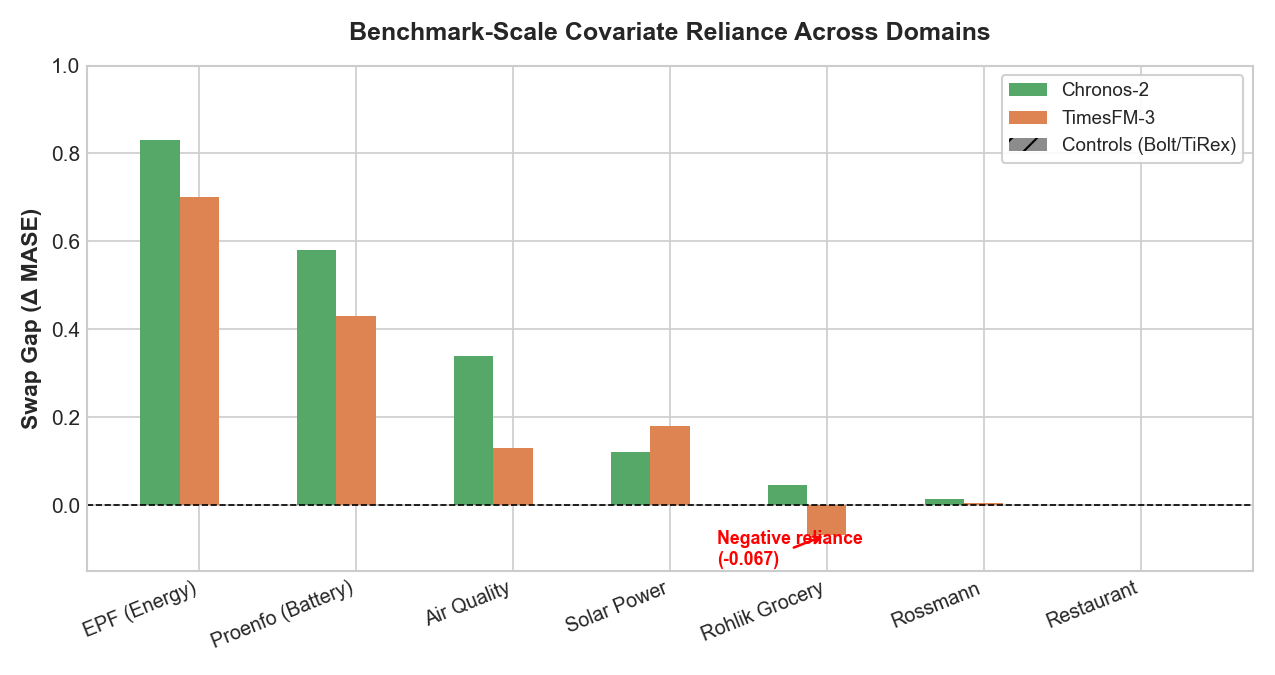
\includegraphics[width=0.8\textwidth]{study2_domain_reliance.png}
\caption{Domain-level reliance aggregated across models. Energy-price tasks dominate;
retail and static-covariate tasks sit near zero.}
\label{fig:domainagg}
\end{figure*}

\section{Protocol details}
All corruptions are applied at inference time only; the target series, its history,
and the forecast horizon are identical across the intact and corrupted runs, and the
intact prediction is seed-invariant by construction because the generator drives only
the corruptions. The derangement is re-drawn up to 100 times so that no series keeps
its own covariates. Known-future columns are swapped only when the benchmark declares
them known; past-only and static columns stay NaN in the future frame and are dropped
by adapters with declared-known semantics (e.g., Chronos-2) or handled by the model's
own featurization (TabPFN-TS). Gaps (store closures) are forward-filled before
probing, with the seed row used to back-fill the first step.

\section{Reproducibility}
The harness, adapters, planted generator, ridge reference, conversions, and unit tests
are self-contained; importing the package never downloads weights or imports a deep
learning framework, and a test enforces this. The GPU-free demo reproduces the
instrument on planted data. A five-seed re-run of five headline cells in a fresh
environment (Python 3.13, fev 0.10, chronos-forecasting 2.3) reproduces the
EPF/Chronos-2 intact MASE to four decimals and is released as
\texttt{seed\_spread\_5seed.csv} (driver: \texttt{scripts/remote/run\_seed\_spread.py}). The full audit is regenerated from the task chunks listed
in Appendix~A with one command per chunk; per-(model, task, seed) gaps are the only
quantities aggregated, and every table and figure in this paper is derived from those
summaries. Metric guards and the exact MASE definition (including the degenerate-scale
NaN rule) are unit-tested.

\end{document}
